%  sample eprint article in LaTeX           --- M. Peskin, 9/7/00
%  modified for LHCP2017, lhcp2017@sjtu.edu.cn
%  This file is part of a tar file, which can be downloaded from the LHCP2017 indico site. 
%   https://indico.cern.ch/event/517784/overview 
% 


\documentclass[10pt]{article}
\usepackage{graphicx}
\usepackage{hyperref}

%particles
\newcommand{\jpsi}{\rm J/$\psi$}
\newcommand{\psip}{$\psi^\prime$}
\newcommand{\jpsiDY}{\rm J/$\psi$\,/\,DY}
\newcommand{\chic}{$\chi_{\rm c}$}
\newcommand{\pip}{$\pi^{+}$}
\newcommand{\pim}{$\pi^{-}$}
\newcommand{\pizero}{$\pi^{0}$}
\newcommand{\kap}{K$^{+}$}
\newcommand{\kam}{K$^{-}$}
\newcommand{\pbar}{$\rm\overline{p}$}
\newcommand{\ccbar}{\ensuremath{\mathrm{c\overline{c}}}}
\newcommand{\bbbar}{\ensuremath{\mathrm{b\overline{b}}}}
\newcommand{\Dzero}{\ensuremath{\mathrm{D^{0}}}}
\newcommand{\Dzerobar}{\ensuremath{\mathrm{\overline{D}^{0}}}}
\newcommand{\Dpm}{\ensuremath{\mathrm{D^{\pm}}}}
\newcommand{\Ds}{\ensuremath{\mathrm{D_{s}^{\pm}}}}
\newcommand{\Dstar}{\ensuremath{\mathrm{D^{*\pm}}}}

%collision systems
\newcommand{\pp}{pp}
\newcommand{\pPb}{p--Pb}
\newcommand{\PbPb}{Pb--Pb}

%detectors
\newcommand{\ezdc}{$E_{\rm ZDC}$}

%units
\newcommand{\GeVc}{GeV/$c$}
\newcommand{\GeVcsq}{GeV/$c^2$}

%others
\newcommand{\degree}{$^{\rm o}$}
\newcommand{\s}{\ensuremath{\sqrt{s}}}
\newcommand{\snn}{\ensuremath{\sqrt{s_{\rm NN}}}}
\newcommand{\y}{\ensuremath{y}}
\newcommand{\pt}{\ensuremath{p_{\rm T}}}
\newcommand{\dedx}{d$E$/d$x$}
\newcommand{\dndy}{d$N$/d$y$}
\newcommand{\dndydpt}{${\rm d}^2N/({\rm d}y {\rm d}p_{\rm t})$}
\newcommand{\zpar}{\ensuremath{z_{||}}}
\newcommand{\zpargen}{\ensuremath{z_{||}^{\mathrm{part}}}}
\newcommand{\zpardet}{\ensuremath{z_{||}^{\mathrm{det}}}}
\newcommand{\ptchjet}{\ensuremath{p_{\mathrm{T,ch\, jet}}}}
\newcommand{\ptjet}{\ensuremath{p_{\mathrm{T,jet}}}}
\newcommand{\ptchjetgen}{\ensuremath{p_{\mathrm{T,ch\,jet}}^{\mathrm{part}}}}
\newcommand{\ptchjetdet}{\ensuremath{p_{\mathrm{T,ch\,jet}}^{\mathrm{det}}}}
\newcommand{\ptd}{\ensuremath{p_{\mathrm{T,D}}}}
\newcommand{\ptdgen}{\ensuremath{p_{\mathrm{T,D}}^{\mathrm{part}}}}
\newcommand{\ptddet}{\ensuremath{p_{\mathrm{T,D}}^{\mathrm{det}}}}
\newcommand{\antikt}{anti-\ensuremath{k_{\mathrm{T}}}}
\newcommand{\Antikt}{Anti-\ensuremath{k_{\mathrm{T}}}}
\newcommand{\kt}{\ensuremath{k_{\mathrm{T}}}}
\newcommand{\pthard}{\ensuremath{p_{\mathrm{T,hard}}}}



%%%%%%%%%%%%%%%%%%%%%%%%%%%%%%%%%%%%%%%%%%%%%%%%%%%%%%%%%%%%%%%%%%%%%%%%%%%%
%   document style macros
%%%%%%%%%%%%%%%%%%%%%%%%%%%%%%%%%%%%%%%%%%%%%%%%%%%%%%%%%%%%%%%%%%%%%%%%%%%%
\def\Title#1{\begin{center} {\Large #1 } \end{center}}
\def\Author#1{\begin{center}{ \sc #1} \end{center}}
\def\Address#1{\begin{center}{ \it #1} \end{center}}
\def\andauth{\begin{center}{and} \end{center}}
\def\submit#1{\begin{center}Submitted to {\sl #1} \end{center}}
\newcommand\pubblock{\rightline{\begin{tabular}{l} Proceedings of the Fifth Annual LHCP\\ \pubnumber\\
         \pubdate  \end{tabular}}}

\newenvironment{Abstract}{\begin{quotation} \begin{center} 
             \large ABSTRACT \end{center}\bigskip 
      \begin{center}\begin{large}}{\end{large}\end{center} \end{quotation}}

\newenvironment{Presented}{\begin{quotation} \begin{center} 
             PRESENTED AT\end{center}\bigskip 
      \begin{center}\begin{large}}{\end{large}\end{center} \end{quotation}}

\def\Acknowledgements{\bigskip  \bigskip \begin{center} \begin{large}
             \bf ACKNOWLEDGEMENTS \end{large}\end{center}}
%%%%%%%%%%%%%%%%%%%%%%%%%%%%%%%%%%%%%%%%%%%%%%%%%%%%%%%%%%%%%%%%%%%%%%%%%%%%
%  personal abbreviations and macros
%    the following package contains macros used in this document:
\input econfmacros.tex
%%%%%%%%%%%%%%%%%%%%%%%%%%%%%%%%%%%%%%%%%%%%%%%%%%%%%%%%%%%%%%%%%%%%%%%%%%%

\textwidth=6.5in  \textheight=8.75in
\hoffset=-.85in
\voffset=-0.6in

%%  DO NOT CHANGE anything above.

% include packages you will need
\usepackage{color}

%%%%%%%%%%%%%%%%%%%%%%%%%%%%%%%%%%%%%%%%%%%%%%%%%%%%%%%%%%%%%%%%%%%%
% basic data for the eprint:
%%%%%%%%%%%%%%%%%%%%%%%%%%%%%%%%%%%%%%%%%%%%%%%%%%%%%%%%%%%%%%%%%%%%

% Instruction:
% Please change each of the following fields:
%

%% preprint number data:
% If there is a preprint number from your institute, or experiment note number, please fill it in 
%\newcommand\pubnumber{ ATL-PHYS-PROC-2017-XXX }
\newcommand\pubnumber{ }

%% date
\newcommand\pubdate{\today}

%%  Affiliation
\def\affiliation{
On behalf of the ALICE Collaboration, \\
Physics Department, \\
Yale University, New Haven, CT 06511, USA}

%% Acknowledge the support
\def\support{\footnote{Work supported by the U.S. Department of Energy under grant number DE-SC0004168.}}

\begin{document}

% large size for the first page
\large
\begin{titlepage}
\pubblock


%% Change the title, name, abstract
%% Title 
\vfill
\Title{New results on jets and heavy flavor in heavy-ion collisions with ALICE}
\vfill

%  if you need to add the support use this, fill the \support definition above. 
%   \Author{ FIRSTNAME LASTNAME \support }
\Author{Salvatore Aiola\support}
\Address{\affiliation}
\vfill
\begin{Abstract}

here it goes

\end{Abstract}
\vfill

% DO NOT CHANGE 
\begin{Presented}
The Fifth Annual Conference\\
 on Large Hadron Collider Physics \\
Shanghai Jiao Tong University, Shanghai, China\\ 
May 15-20, 2017
\end{Presented}
\vfill
\end{titlepage}
\def\thefootnote{\fnsymbol{footnote}}
\setcounter{footnote}{0}
%

% normal size for the rest
\normalsize 

%% Your paper should be entered below. 

\section{Introduction}
A comprehensive and far-reaching heavy-ion programme is part of the scientific goals of the CERN Large Hadron Collider.
The large statistics accumulated during the LHC Run-1 and Run-2 have given access to an unprecedented number of observables connected to rare high-$Q^2$ processes.
Such hard probes are rare enough to be singled out from the large bulk of particles produced in ultra-relativistic heavy-ion collision. By interacting with the Quark-Gluon Plasma (QGP) these self-produced probes
can carry crucial pieces of information about the transport properties of the QGP.

The suppression of the jet production cross section in ultra-relativistic heavy-ion collisions has been established both at RHIC~\cite{STAR:2017a} and at the LHC~\cite{ALICE:2015a}. The suppression is interpreted as the result of the interaction of the hard-scattered partons 
with the QGP, which dampens the momentum of the hard parton via radiative and collisional energy loss (\emph{jet quenching}). A number of theoretical models, such as JEWEL and YaJEM, can effectively reproduce
the data; however the exact determination of the parameters of the energy loss as well as the details of the energy-loss mechanism are still pending. Some additional constraints come from the observation (or lack thereof) of
the modification of the internal structure of the jets. A number of observable has been proposed. The ALICE Collaboration is active in this area and some of the latest results have been presented at this conference.

Heavy-flavor (charm and beauty) particles have been used as probes of the QGP both at RHIC and at the LHC. What makes heavy-flavor partons special is their non-zero mass which plays the role of a second hard scale, independent of the momentum.
As a consequence, they can be singled out from the bulk even at low momentum. Furthermore, perturbative Quantum Chromo-Dynamics (pQCD) methods are effective in calculating the production cross-section in vacuum, i.e. in \pp\ collisions, down to zero momentum, notwithstanding large uncertainties.
The production cross section of open-charm mesons has been observed to be suppressed at about the same level as in the light-flavor case. Earlier theoretical predictions showed smaller suppression, however improvements in the theoretical models 
have reduced the discrepancy between theory and experiments. The measured azimuthal anisotropy of D mesons (the elliptic flow measured via the second coefficient $v_2$ of the Fourier decomposition) has played an important role in challenging
the theoretical models. Hidden-charm mesons have an equally important role in the characterisation of the QGP.
The observed \jpsi\ yield in heavy-ion collision has been interpreted as being the result of two competing effects: dissociation of the \ccbar\ pairs in the QGP; and generation in the QGP from pairs of charm and anti-charm quarks coming from independent scatterings.
The \jpsi\ generated in the QGP is expected to flow with the QGP medium, therefore a precise measurement of the \jpsi\ elliptic flow is crucial.
At this conference the ALICE Collaboration has presented an updated measurement of the $v_2$ of D mesons as well as \jpsi, using the larger statistical samples available from Run-2.

In recent years, collective effects usually associated with the formation of the QGP have been observed in a subset of \pPb\ and in \pp\ collisions, characterised by a very large event multiplicity. These observations could be taken as indication that the smallest drop
of QGP is formed in such collisions, however no unambiguous proof has been shown yet. In particular no unexpected effects have been observed using hard probes (jets or heavy-flavor particles). In these proceedings we present two recent measurements from ALICE.

\section{\PbPb\ collisions}

\subsection{Jet Substructure}

\begin{figure}[htb]
\centering
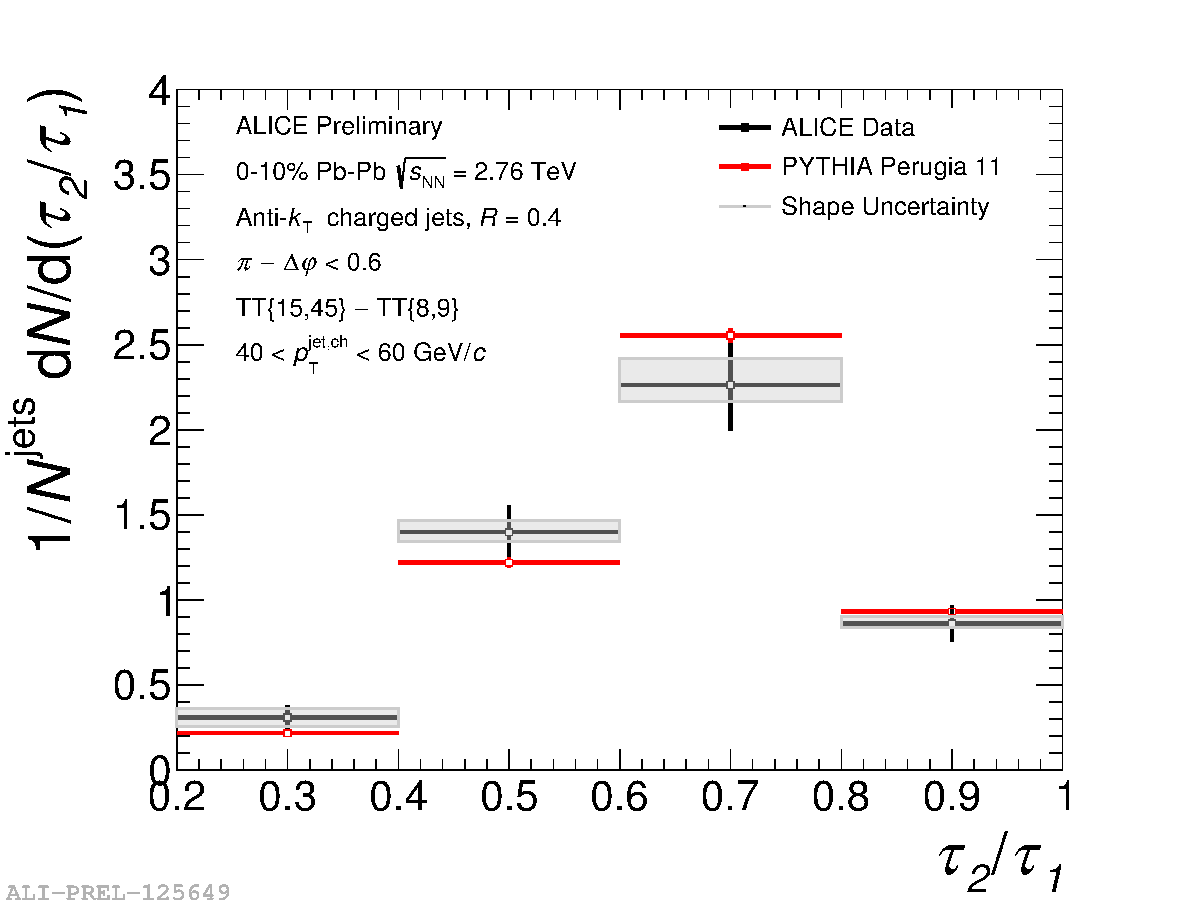
\includegraphics[width=.5\textwidth]{img/2017-Feb-03-Tau2to1_40to60_Full_Results_0}
\caption{Nsubjettiness}
\label{fig:nsubjettiness}
\end{figure}


\subsection{Heavy-Flavor Elliptic Flow}

\section{\pPb\ collisions}

\subsection{Hadron-Jet Cross Section}

\subsection{Jet Substructure}

 
%%%%%%%%%%%%%%%%%%%%%%%%%%%%%%%%%%%%%%%%%%%%%%%%%%%%%%%%%%%%%%%%%%%%%%%%%
%%
%%   use this format to include an .eps figure into your paper
%%
%\begin{figure}[htb]
%\centering
%\includegraphics[height=2in]{head_lhcp2017.jpg}
%\caption{ Place the caption here}
%\label{fig:figure1}
%\end{figure}
%%%%%%%%%%%%%%%%%%%%%%%%%%%%%%%%%%%%%%%%%%%%%%%%%%%%%%%%%%%%%%%%%%%%%%%%%%%

%%%%%%%%%%%%%%%%%%%%%%%%%%%%%%%%%%%%%%%%%%%%%%%%%%%%%%%%%%%%%%%%%%%%%%%%%
%%
%%   use this format to include a LaTeX table  into your paper
%%
%\begin{table}[t]
%\begin{center}
%\begin{tabular}{l|ccc}  
%Patient &  Initial level($\mu$g/cc) &  w. Magnet &  
%w. Magnet and Sound \\ \hline
%Guglielmo B.  &   0.12     &     0.10      &     0.001  \\
%Ferrando di N. &  0.15     &     0.11      &  $< 0.0005$ \\ \hline
%\end{tabular}
%\caption{ place the caption here }
%\label{tab:table1}
%\end{center}
%\end{table}
%%%%%%%%%%%%%%%%%%%%%%%%%%%%%%%%%%%%%%%%%%%%%%%%%%%%%%%%%%%%%%%%%%%%%%%%%%%


%%  if necessary
%\Acknowledgements
%I am grateful to XYZ for fruitful discussions.

\bibliography{biblio}{}
\bibliographystyle{iopart-num}
 
\end{document}

